\documentclass[12pt,a4paper,twoside]{report}
\usepackage[T1]{fontenc} 
\usepackage[french]{babel}
\usepackage[ansinew,utf8]{inputenc}

\usepackage{graphicx}
\usepackage{color}
\usepackage{rotating}
%\usepackage[top=2.5cm,bottom=2cm,left=2.5cm,right=2cm]{geometry}
\usepackage[left=1.3in,right=1in,top=1in,bottom=1in]{geometry}
\usepackage{caption}
\linespread{1.1}
\usepackage{setspace}
\usepackage{microtype}
\usepackage{gensymb}
\usepackage[toc,page]{appendix}
\usepackage{textcomp}
\usepackage{makeidx}
\usepackage{multirow}
\usepackage[french]{minitoc}
\setcounter{minitocdepth}{1}
\usepackage{eurosym}
\definecolor{gray}{rgb}{.7,.7,.7}
\definecolor{Prune}{RGB}{99,0,60}
\usepackage[dvipsnames]{xcolor}
\usepackage{mdframed}
\usepackage{lmodern}
\usepackage{subfig}
\usepackage[Lenny]{fncychap}
\usepackage{calc}
\usepackage{float}
\usepackage{booktabs}
\usepackage{epstopdf}
\usepackage{pgf,tikz}
\usepackage{schemabloc}
\usepackage{caption}
\usetikzlibrary{circuits}
\usepackage{amsmath,amssymb,amsfonts,amsbsy}
\usepackage{dsfont,pifont} 
\usepackage{nopageno}
\usepackage{mdframed}
\usepackage{multirow} %% Pour mettre un texte sur plusieurs rangées
\usepackage{multicol} %% Pour mettre un texte sur plusieurs colonnes
%\usepackage{scrextend} %Forcer la 4eme  de couverture en page pair
\usepackage{textpos}

\usepackage{fancyhdr}
\usepackage{fancybox}

\pagestyle{fancy}
\usepackage{lastpage}
\usepackage[pdftex,letterpaper,colorlinks=true,linkcolor=blue]{hyperref}
\fancyhead[LE,RO]{\bfseries\thepage}    % Page number (boldface) in left on even
% pages and right on odd pages
\fancyhead[RE]{\it\nouppercase{\leftmark}}      % Chapter in the right on even pages
\fancyhead[LO]{\it\nouppercase{\rightmark}}     % Section in the left on odd pages

\rfoot{}
\cfoot{}
\lfoot{}

\usepackage[french]{minitoc} 
\setcounter{minitocdepth}{1}

\newcommand{\clearemptydoublepage}{\newpage{\pagestyle{empty}\cleardoublepage}}

\usepackage{pdfpages}

\makeindex
\begin{document}

\dominitoc

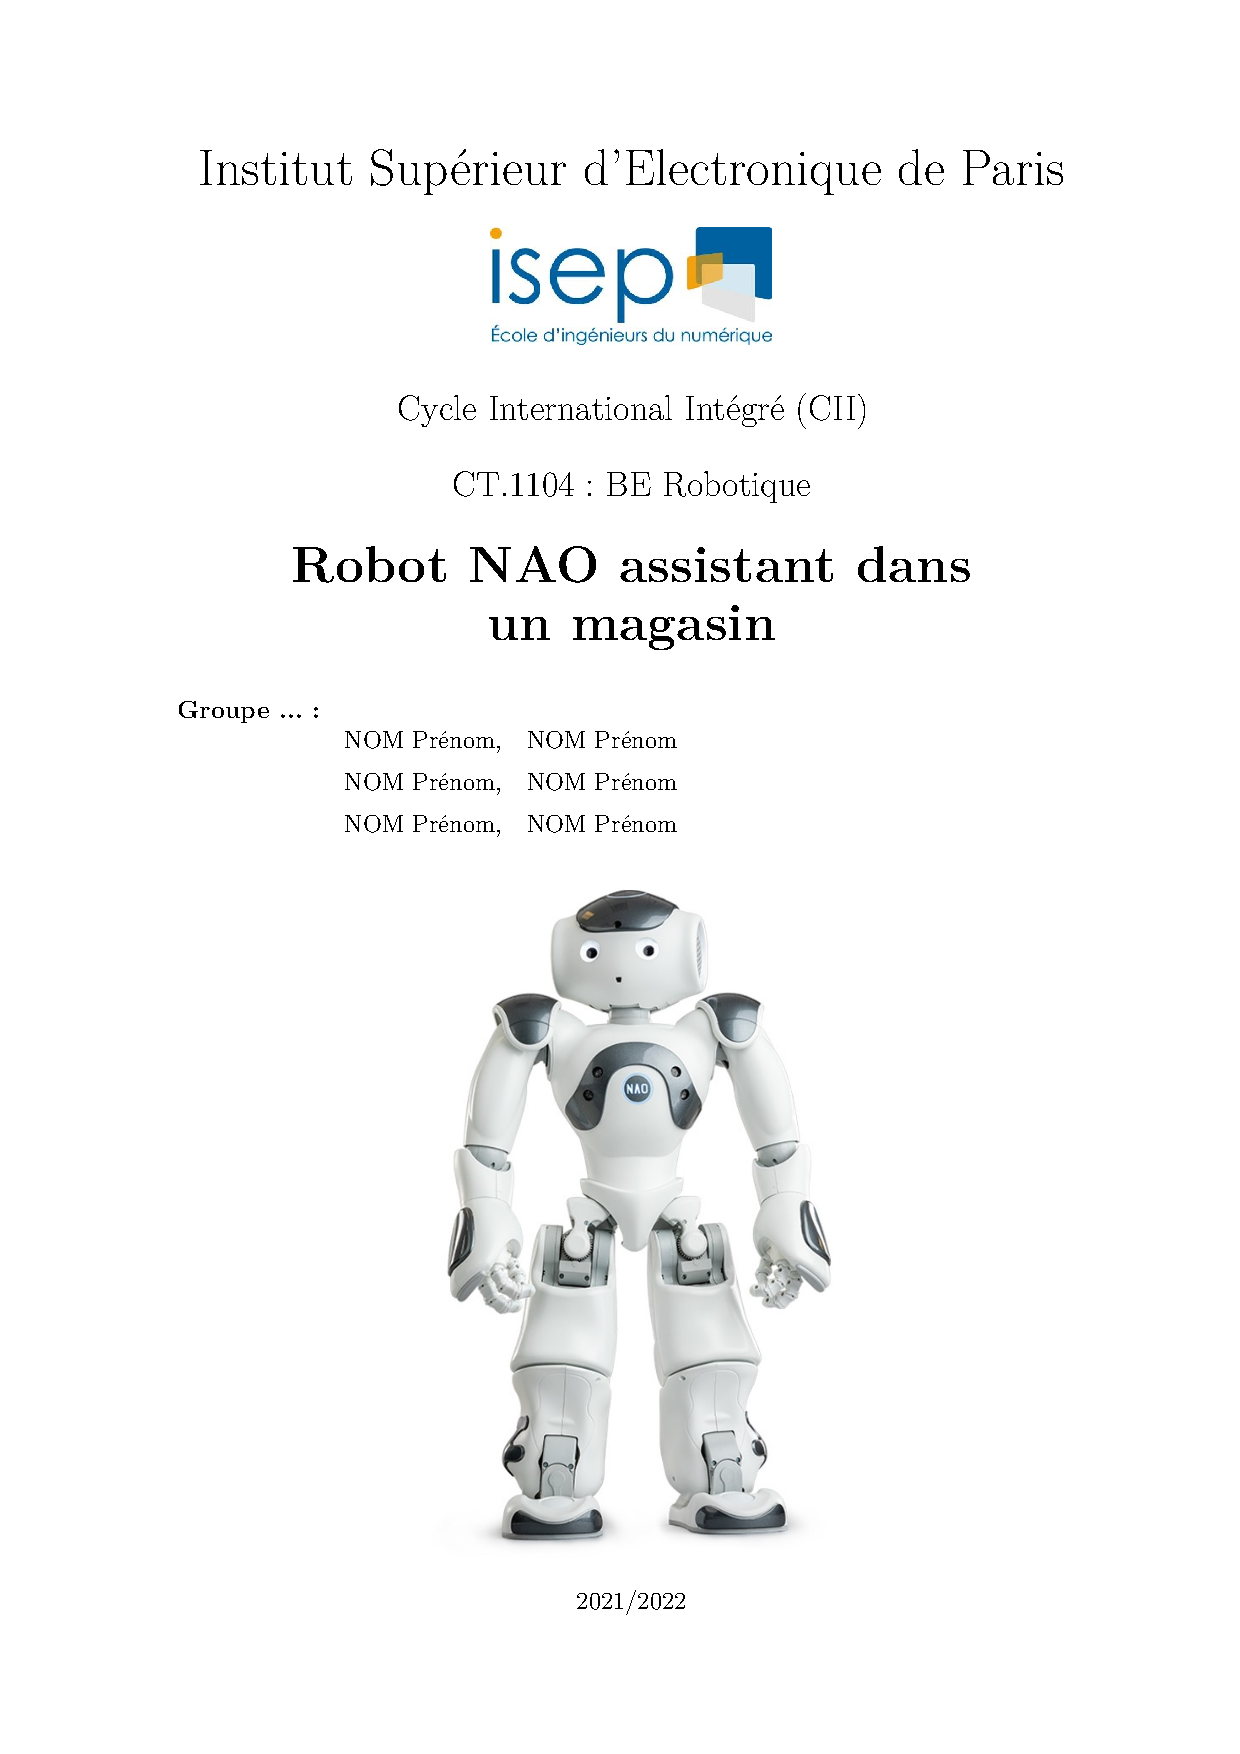
\includepdf{Page_garde.pdf}
\clearemptydoublepage
%\includepdf{Page_vide.pdf}
\pagenumbering{roman}
\tableofcontents
\listoffigures
\listoftables

\clearemptydoublepage
\pagenumbering{arabic}

\addstarredchapter{Introduction}
\chapter*{Introduction \label{Sec:Intro}}

\subsection*{Contexte du sujet}
De nos jours, plusieurs secteurs de l'industrie reposent sur l'utilisation des robots manipulateurs (industriels), comme c'est le cas dans l'industrie automobile ou dans la construction navale. Plusieurs tâches ont été confiées à des robots, comme le transport de pièces, la manipulation, l'assemblage, la soudure ou encore la peinture. Ce type d'industrie nécessite fréquemment la manipulation de pièces massives et volumineuses. Par conséquent, les robots utilisés sont de grandes dimensions et possèdent des capacités importantes, que ce soit en terme de volume de travail, de vitesse de déplacement, de précision des mouvements ou bien en terme de charge utile.

\subsection*{Travail réalisé}
Afin de répondre à cet objectif, nous avons d'abord focalisé notre attention sur l'obtention d'un modèle dynamique du robot manipulateur série à six axes \verb"DENSO VP-6242G", évoluant dans l'espace tridimensionnel. Chaque axe est considéré comme réalisant une liaison pivot (encore appelée \emph{liaison rotoïde}) entre deux bras du robot, une liaison mécaniquement imparfaite compte tenu de la présence non négligeable de frottement dans toutes les liaisons. 
Chaque bras est supposé constitué d'un solide rigide. Pour cela, nous avons commencé par la construction d'un modèle analytique décrivant la position et l'orientation de l'organe terminal à partir des coordonnées articulaires. Ce modèle, dit Modèle Géométrique Direct (MGD), ne dépend que de paramètres géométriques qui sont connus. 

\subsection*{Structure du rapport}
........

\chapter{Généralités sur le concept de co-manipulation Homme-Robot \label{Chapitre_1}}
\minitoc

La collaboration entre les humains et les robots est de plus en plus recommandée dans plusieurs domaines, y compris le domaine de l'industrie. Dans ce chapitre, nous allons aborder le contexte de la co-manipulation homme-robot. Nous expliquerons d'abord la nécessité d'une coopération entre un robot et un être humain. Comme il y a plusieurs façons de faire coopérer un homme avec un robot, nous exposerons les différents types de coopération pouvant exister. Les différentes solutions existantes et les problèmes d'une co-manipulation homme-robot seront aussi discutés. Enfin, nous présenterons le problème de co-manipulation tel que nous l'abordons, et sa mise en perspective avec les autres approches similaires.

\section{Définition}
En robotique, la co-manipulation consiste à réaliser une tâche précise, d'une façon conjointe par un robot et un être humain (co-manipulation homme-robot), ou bien par deux robots (co-manipulation robot-robot). Nous pouvons donc avancer qu'une co-manipulation nécessite le partage de l'espace de travail, mais aussi le moment d'intervention. La co-manipulation homme-robot a pour objectif de profiter des capacités des robots (force, précision, \ldots) et de la capacité décisionnelle des humains pour réaliser des tâches.

Dans cette étude, nous nous intéressons à la co-manipulation homme-robot destinée au secteur industriel. En industrie automobile par exemple, elle peut intervenir pour des tâches de montage, d'assemblage ou  de déplacement de charges lourdes.


\section{Nécessité de la co-manipulation}
Depuis leur apparition, les robots sont de plus en plus présents dans différents secteurs économiques, notamment dans le domaine de l'industrie, mais aussi en chirurgie, en médecine de la rééducation, en agriculture, en construction, dans le domaine des services, de transport, \emph{etc}. Pour des raisons de rapidité, de précision, et parfois de sécurité, les robots ont permis de remplacer l'être humain pour réaliser beaucoup de tâches comme dans les chaînes de production ou bien pour l'intervention dans des milieux dangereux ou même difficilement accessibles par l'être humain.

Dans le secteur industriel, la robotisation des chaînes de production a permis d'augmenter la productivité grâce aux capacités des robots manipulateurs modernes, aussi bien en terme de vitesse qu'en terme de précision ou d'endurance. De plus, la manipulation de charges lourdes nécessite une force importante qui ne peut, la plupart du temps, qu'être assurée par des robots. Ces avantages ont permis d'optimiser le temps de production, d'avoir des produits de qualité, et d'exempter l'opérateur humain de la nécessité de produire des efforts importants.

Cependant, les tâches compliquées sont difficilement achevées par les robots, notamment la manipulation des pièces de dimensions différentes, ou dans un environnement sous contraintes imprévues et non modélisées. La décision limitée des robots dans ces cas peut conduire non seulement à ne pas accomplir la tâche, mais peut aussi entraîner des dégâts matériels. Par ailleurs, un opérateur humain peut générer des décisions beaucoup plus appropriées qu'un robot, lors de la manipulation des pièces de caractéristiques géométriques dissemblables, surtout si elle se fait dans un environnement sous contraintes dynamiques.

De ce qui précède, nous pouvons conclure qu'une co-manipulation homme-robot est indispensable dans le secteur industriel. Néanmoins, pour une collaboration entre un robot et un être humain, le contrôle du robot doit être maîtrisé, afin de garantir la sécurité de l'opérateur, qui est en contact direct avec le robot, tout en s'assurant que les deux accomplissent la tâche correctement.

\chapter{Modélisation des robots manipulateurs} \label{Chapitre_2}
\minitoc

Dans ce chapitre, nous allons commencer par présenter la manière d'obtenir la structure mathématique paramétrée d'un MDI, puis nous présenterons la manière d'obtenir une estimation de ses paramètres par le biais de l'identification de ce modèle, à partir de données expérimentales. %
L'obtention d'un MDI nécessite au préalable de construire les modèles géométrique et cinématique directs (respectivement MGD et MCD). La construction du MGD consiste à déterminer les équations définissant la position et l'orientation de l'organe terminal, exprimées dans un repère fixe, à partir des coordonnées articulaires de position et des paramètres géométriques du robot. La construction du MCD consiste quant à elle à déterminer les équations définissant la vitesse linéaire et la vitesse angulaire de l'organe terminal, exprimées dans un repère fixe, à partir des coordonnées articulaires de position et de vitesse ainsi que des paramètres géométriques du robot.
Ces derniers correspondent aux différents angles et distances entre deux repères consécutifs attachés aux corps du robot.
\par
Ce chapitre est organisé de la manière suivante. La section \ref{Model_robot} présente les outils mathématiques permettant l'obtention du MDI. La section \ref{Model_denso} correspond à l'application de ces outils au cas du robot \verb"DENSO VP-6242G". Dans la section \ref{Ident_denso}, nous focaliserons la présentation sur la démarche d'identification d'un MDI à partir de données expérimentales. Pour finir, la section \ref{Ident_denso} permettra d'appliquer cette démarche au cas du robot \verb"DENSO VP-6242G".

\section{Modèle géométrique direct}
\label{Model_robot}
Considérons le cas d'un robot à $n$ articulations rotoïdes. A chaque corps $i$, est attaché un repère $R_i$, dont l'axe $z_i$ est porté par l'axe de rotation de l'articulation. On définit aussi un repère de base $R_0$ qui est immobile. Il correspond à un repère galiléen. L'un des choix de ce repère est qu'il soit confondu avec le repère $R_1$ quand la variable articulaire $q_1$ est nulle.
%Le repère attaché à l'organe terminal $R_{ee}$ (end-effector en anglais), est choisi aussi confondu avec $R_n$ et soumis à une translation jusqu'au centre de gravité de l'organe terminal.
Ce choix nous permet de minimiser le nombre des paramètres géométriques non nuls. Aussi, comme il n'y a pas d'articulation entre le dernier corps du robot et l'organe terminal, le repère $R_n$ s'attache à ces deux corps.

\subsection{Convention et paramètres de Denavit-Hartenberg Modifiée}
Le calcul du modèle dynamique d'un robot se base sur les paramètres géométriques, connus sous le nom de  \og\textit{paramètres de la convention de Denavit-Hartenberg Modifiée (DHM)}\fg{}. Ces paramètres permettent de définir la position et l'orientation d'un repère $R_i$ dans $R_{i-1}$. La figure \ref{MDH} illustre les paramètres de la convention DHM :
\begin{figure}[H]
\begin{center}
%\resizebox{12cm}{!}{
\begin{tikzpicture}[scale=1]
\draw[black, ->,>=latex,very thick](0,0)--(0,5);
\draw[black, ->,>=latex,very thick](0,1)--(8,2);
\draw[black, ->,>=latex,very thick](6,1.75)--(4,6);
\draw[black, ->,>=latex,very thick](4.7,4.5)--(8,6);
\draw[red,dashed,>=latex,thick](6,1.75)--(6,4.3);
\draw[red,dashed,>=latex,thick](4.7,4.5)--(8.5,5);
\node(N1)at(3,1.35){\textcolor{blue}{$/$}};
\node(N1)at(6.9,4.75){\textcolor{blue}{$/$}};
\node(N1)at(0,3){\textcolor{blue}{$=$}};
\node(N1)at(6,3.5){\textcolor{blue}{$=$}};
\node(N1)at(-0.5,1.){$O_{i-1}$};
\node(N1)at(-0.6,2){$(R_{i-1})$};
\node(N1)at(4.4,4.5){$O_i$};
\node(N1)at(5.5,5.5){$(R_i)$};
\node(N1)at(8.4,1.9){$x_{i-1}$};
\node(N1)at(8.2,6){$x_i$};
\node(N1)at(0,5.2){$z_{i-1}$};
\node(N1)at(4,6.2){$z_i$};
\node(N1)at(2.6,1.55){$d_i$};
\node(N1)at(5.1,3.1){$r_i$};
\draw[->] (6,2.5) arc (0:160:0.18cm);
\draw[->] (5.75,4.6) arc (0:65:0.3cm);
\node(N1)at(5.75,2.85){$\alpha_i$};
\node(N1)at(6,4.8){$\theta_i$};
\end{tikzpicture}
%}
\end{center}
\caption{Convention de Denavit-Hartenberg Modifiée.}
\label{MDH}
\end{figure}
En se basant sur la figure \ref{MDH}, nous définissons les paramètres suivants :
\begin{equation}
\left\{
\begin{array}{l}
\alpha_i = \widehat{z_{i-1},z_i} /x_{i-1} \\
d_i = \overline{O_{i-1},z_i} / x_{i-1} \\
r_i = \overline{x_{i-1},O_i} / z_i \\
\theta_i = \widehat{x_{i-1},x_i} /z_i \\
\end{array}
\right.
\label{DH}
\end{equation}
Tel que:
\begin{itemize}
\item[•] $z_{i-1}$ : est porté par l'axe de l'articulation $i-1$;
\item[•] $x_{i-1}$ : est porté par la perpendiculaire entre les axes $z_{i-1}$ et $z_i$. Si $z_{i-1}$ et $z_i$ se coupent, $x_{i-1}$ est alors dirigé perpendiculairement au plan formé par les deux axes;
\item[•] $O_{i-1}$ : résulte de l'intersection de la perpendiculaire entre $z_i$ et $z_{i-1}$ avec ce dernier;
\item[•] $r_i$ : est la variable articulaire pour les articulations prismatiques;
\item[•] $\theta$ : est la variable articulaire pour les articulations rotoïdes;
\item[•] $d_i$ : est la distance entre $O_{i-1}$ et $z_i$ selon l'axe $x_{i-1}$.
\end{itemize}

%\newpage

\section{Modélisation du robot \texttt{Denso VP-6242G}}
\label{Model_denso}
\subsection{Description du robot \texttt{Denso VP-6242G} et de son module de contrôle}
Le robot \verb"Denso VP-6242G" est un robot conçu et fabriqué par la firme japonaise \textit{Denso}. Il est destiné à des tâches d'assemblage et de manutention nécessitant un espace réduit et une capacité relativement faible, dans différents secteurs comme celui de l'électronique, l'agro-alimentaire, l'industrie pharmaceutique, la plasturgie \emph{etc}. Ce robot possède six articulations rotoïdes. Il pèse environ $15$ $kg$ et sa charge utile est de $2$ $kg$. La figure \ref{VP-6242G} présente le robot \verb"Denso VP-6242G" dont nous disposons au laboratoire.
\begin{center}
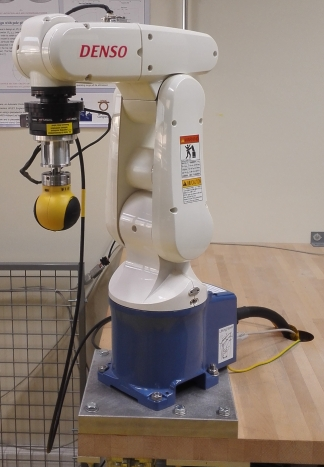
\includegraphics[scale=0.6]{Robot_TroisQuart_Red.jpg}
\captionof{figure}{Le robot \texttt{Denso VP-6242G} équipé d'un capteur de force et d'un outil.}
\label{VP-6242G}
\end{center}
%\begin{center}
%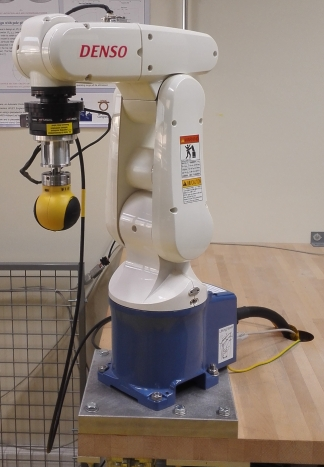
\includegraphics[clip,scale=0.58]{Robot_TroisQuart_Red.jpg}}
%\caption{\label{VP-6242G} Le robot \texttt{Denso VP-6242G} équipé d'un capteur de force et d'une outil.}
%\end{center}
Comme l'indique les deux photos de la figure \ref{VP-6242G}, le robot est équipé d'un capteur de force de type \texttt{Gamma} distribué par la société \textit{ATI Industrial Automation}.
%\textbf{Sensing range :} The sensing range of a sensor is a region where every event that takes place in this region can be detected.
%is the area between the minimum and the maximum sensing limits.
%\textbf{Resoluion :} The resolution of a sensor is the smallest change it can detect in the quantity that it is measuring.
Le capteur est fixé sur le corps de la dernière articulation du robot (figure \ref{fig:capteur_force}). Un outil sphérique est installé sur le capteur de force (figure \ref{fig:poignee}). La masse totale du capteur avec l'outil est $m_t = 0.94$ $kg$. Cette installation robotique doit permettre d'utiliser ce robot pour des essais expérimentaux de co-manipulation homme-robot.  Le but de ces essais expérimentaux est de faire la démonstration de la faisabilité de notre approche pour la co-manipulation homme-robot en vue de la manutention de charges lourdes.
%\begin{center}
%\includegraphics[scale=0.55]{capteur_poignee.jpg}
%\captionof{figure}{Le capteur de force (B), l'outil installé (A) et le module de contrôle (C).}
%\label{poignee_capteur}
%\end{center}
\begin{figure}[h!]
\subfloat[\label{fig:capteur_force}]{
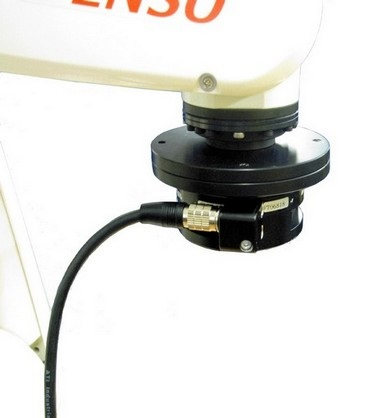
\includegraphics[clip,scale=0.55]{capteur_force.jpg}}
\hspace{0.2cm}
\subfloat[\label{fig:poignee}]{
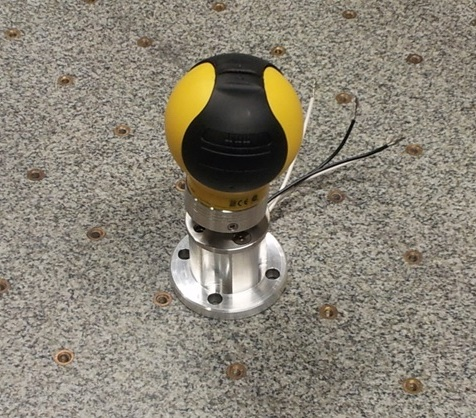
\includegraphics[clip,scale=0.55]{poignee.jpg}}
\hspace{0.2cm}
\subfloat[\label{fig:Controlleur}]{
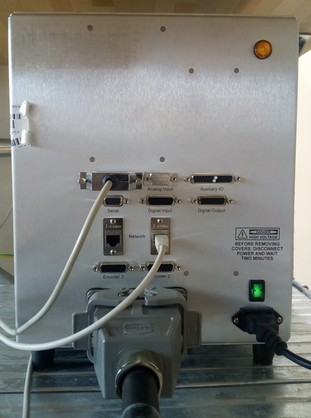
\includegraphics[clip,scale=0.33]{Controlleur.jpg}}
\caption{\label{poignee_capteur} Le capteur de force (a), l'outil installé (b) et le module de contrôle (c).}
\end{figure} \\
Au laboratoire, le robot \verb"Denso" est disponible avec un module de contrôle à architecture ouverte de la société \textit{Quanser} (figure \ref{fig:Controlleur}). Le système robot + module de contrôle permet d'avoir les capacités d'un système industriel interfacé avec le logiciel de contrôle en temps réel \verb"Quarc", compatible avec \verb"Matlab/Simulink". Le bras robotique contient six encodeurs qui permettent de mesurer les positions angulaires des six arbres de chaque axe (moto-réducteur). Les longueurs des corps constituant le robot sont indiquées dans la figure \ref{RobotFrames}. Pour plus de détails techniques sur ce robot, son module de contrôle et son l'interface, se référer aux sites web.
La communication avec le robot se fait via l'interface \verb"Quarc" dans \verb"Simulink" à travers les blocs \verb"Denso Read" et \verb"Denso Write" (figure \ref{read-write}).
\begin{center}
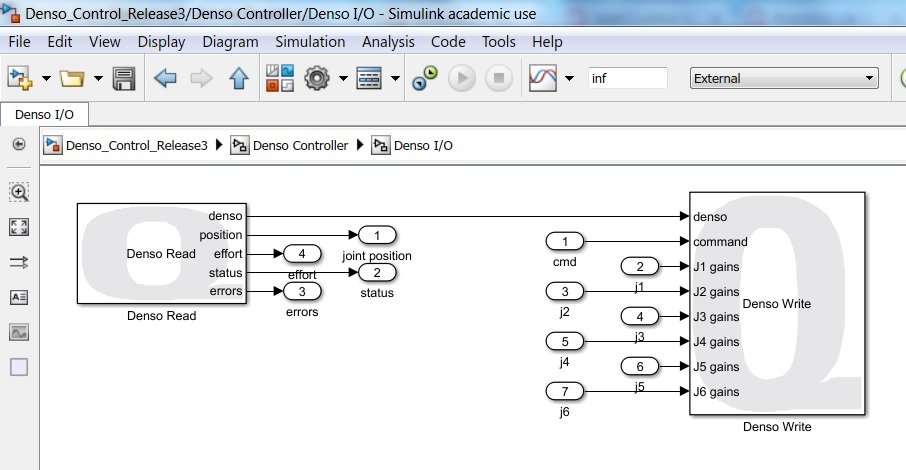
\includegraphics[scale=0.7]{Read-Write.jpg}
\captionof{figure}{Les blocs \texttt{Denso Read} et \texttt{Write}.}
\label{read-write}
\end{center}
Ces blocs fonctionnent à une fréquence d'échantillonnage de $1$ $ms$. Le bloc \verb"Denso Read" permet de nous communiquer les positions des encodeurs articulaires, qui sont, après calibration, transformés en degrés. Le bloc \verb"Denso Read" permet aussi de récupérer la mesure du courant électrique consommé pour chaque moteur, des codes informant sur l'état du robot et de son contrôleur (déconnecté, erreur, normal, ...) et un code d'erreur pour chaque axe. Le bloc \verb"Denso Write" est utilisé pour envoyer des signaux de commande en position/vitesse ou en couple au robot.
Il est possible de commander le robot à travers deux modes : en position/vitesse (entrée 1 du bloc \verb"Denso Write") ou en couple (entrées 2 à 7).

\begin{table}[H]
\caption{Paramètres de la convention DHM correspondant au robot \texttt{Denso VP-6242G}.}
\centering
\begin{tabular}{c||c|c|c|c||c||c|c|c|c}
\toprule
\midrule
$i$ & $\alpha_i$ & $d_i$ & $r_i$ & $\theta_i$ & $i$ & $\alpha_i$ & $d_i$ & $r_i$ & $\theta_i$ \\
\midrule
\midrule
$1$ & $0$ & $0$ & $l_{1z}$ & $q_1$ & $4$ & $- \displaystyle \frac{\pi}{2}$ & $- l_{3x}$ & $l_{3z} + l_4$ & $q_4$ \\
\midrule
$2$ & $\displaystyle \frac{\pi}{2}$ & $0$ & $0$ & $q_2 + \displaystyle \frac{\pi}{2}$ & $5$ & $\displaystyle \frac{\pi}{2}$ & $0$ & $0$ & $q_5$ \\
\midrule
$3$ & $0$ & $l_2$ & $0$ & $q_3 - \displaystyle \frac{\pi}{2}$ & $6$ & $- \displaystyle \frac{\pi}{2}$ & $0$ & $l_5$ & $q_6$ \\
\midrule
\bottomrule
\end{tabular}
\label{tab:MDH}
\end{table}

Pour le premier mode, si la position désirée est constante, donc il s'agit d'une commande en position. Si les positions articulaires désirées évoluent au cours du temps, le signal de commande est la variation de la position désirée. Comme cette variation est appliquée à chaque pas de temps ($1$ $ms$), elle est équivalente à une commande en vitesse. Pour commander le robot en couple, il faut lui appliquer le signal de couple désiré pour chaque axe, qui sera par la suite converti en courant électrique désiré.


\chapter{Identification des paramètres dynamiques d'un robot} \label{Chapitre_2}
\minitoc

Dans le domaine de la commande des systèmes, la plupart des commandes développées nécessitent la connaissance des valeurs numériques des paramètres qui décrivent la dynamique du système.
L'identification est une technique qui permet de trouver une estimation des valeurs de ces paramètres. En parallèle de son importance, l'identification n'est pas une tâche facile, étant donnés les problèmes que nous avons rencontrés durant cette étape. Dans cette section, nous allons présenter en quoi consiste l'identification des paramètres dynamiques pour des robots manipulateurs et comment s'y prendre.

\section{Modèle dynamique pour l'identification}
\label{Ident_denso}

Le modèle dynamique destiné à l'identification est une ré-écriture de l'équation \eqref{MDI5}, sous la forme d'une relation linéaire en les paramètres à identifier, regroupés dans un vecteur noté $\theta$ de dimension ($n_\theta \times 1$) :
\begin{equation}
\tau = D(q,\dot{q},\ddot{q}) \theta
\label{Reg1}
\end{equation}
\begin{equation}
\left[
\begin{array}{c}
\tau_1 \\
\tau_2 \\
. \\
. \\
. \\
\tau_n \\
\end{array}
\right] =
\left[
\begin{array}{cccccc}
D_{11} & D_{12} & . & . & . & D_{1n} \\
0 & D_{22} & . & . & . & D_{2n} \\
. & 0 & . & . & . & . \\
. & . & . & . & . & . \\
. & . & . & . & . & . \\
0 & 0 & . & . & 0 & D_{nn} \\
\end{array}
\right]
\left[
\begin{array}{c}
\theta_1 \\
\theta_2 \\
. \\
. \\
. \\
\theta_n \\
\end{array}
\right],
\label{Reg2}
\end{equation}
où $D$ est une matrice de dimension $(n\times n_\theta)$ qui ne dépend que des paramètres géométriques du robot et des coordonnées articulaires $q$, $\dot{q}$ et $\ddot{q}$. Cette matrice est appelée \emph{matrice d'observation}. En utilisant la même notation que celle dans pour une articulation $i$, nous pouvons définir les \textit{paramètres dynamiques} suivants :
\begin{itemize}
\item[•] $xx_i$, $xy_i$, $xz_i$, $yy_i$, $yz_i$, $zz_i$ : ce sont les composantes de la matrice du tenseur d'inertie $^iI_{i}$ (symétrique) autour de l'origine $O_i$ du repère $R_i$ :
$$ ^iI_{i} = \left[ \begin{array}{ccc}
xx_i & xy_i & xz_i \\ xy_i & yy_i & yz_i \\ xz_i & yz_i & zz_i \\
\end{array} \right]. $$
$xx_i$, $yy_i$, $zz_i$ s'appellent les moments d'inertie par rapport aux axes $Ox_i$, $Oy_i$, $Oz_i$, respectivement. $xx_i$, $yy_i$, $zz_i$ sont toujours positifs. $xy_i$, $xz_i$ et $yz_i$ s'appellent les produits d'inertie;
\item[•] $mx_i$, $my_i$, $mz_i $ : ce sont les moments autour les trois axes de $R_i$;
\item[•] $m_i$ est la masse du corps rattaché à l'articulation;
%\item[•] $Ia_i$ est l'inertie du moteur de l'articulation $i$;
\item[•] $Fv_i$, $Fs_i$ sont les coefficients des frottements visqueux et de Coulomb respectivement, pour un modèle de frottement linéaire en ces paramètres.
\end{itemize}
Ces paramètres sont alors regroupés dans le vecteur suivant :
\begin{equation}
\begin{array}{c}
\theta_i := \left[ \begin{array}{ccccccccccccc} xx_i & xy_i & xz_i & yy_i & yz_i & zz_i & mx_i & my_i & mz_i & m_i & Fs_i & Fv_i \end{array} \right]^T,
\end{array}
\label{vect_param}
\end{equation}
où $^T$ indique le transposé. Le vecteur $\theta$ est construit par la concaténation verticale des vecteurs $\theta_i$ $(i = 1,...,n)$. Les dix premiers paramètres sont appelés \textit{paramètres inertiels} de l'articulation $i$, comme indiqué dans.

\section{Vecteur des paramètres inertiels minimaux}
\label{param_minim}
Dans le cadre de l'identification des paramètres d'un robot, nous pouvons nous retrouver confrontés à l'un des deux cas suivants :
\begin{itemize}
\item[•] certains paramètres inertiels, pour certaines configurations n'interviennent pas dans la dynamique du robot. Du coup, ces paramètres ne sont pas identifiables et peuvent être éliminés du vecteur des paramètres à identifier;
\item[•] comme la relation entre le vecteur des paramètres et la matrice d'observation est linéaire, certains paramètres inertiels peuvent avoir les mêmes coefficients, donc pondérés par des expressions identiques dans la matrice d'observation. Il est alors indispensable de regrouper ces paramètres.
\end{itemize}
La matrice d'observation obtenue dans les deux cas n'est pas de rang plein, ce qui ne permet pas de déterminer les valeurs des paramètres d'une manière exacte.
Afin de pouvoir traiter ce problème, il est nécessaire de définir un vecteur des paramètres minimaux à identifier. Pour cela, nous éliminons les paramètres qui n'affectent pas la dynamique du robot et nous regroupons les paramètres qui sont pondérés des m\^emes coefficients. Les travaux se sont intéressés à :
\begin{itemize}
\item[•] la détermination des paramètres qui n'ont pas d'influence sur la dynamique du robot;
\item[•] les conditions de regroupement des paramètres inertiels;
\item[•] les relations qui permettent le regroupement des paramètres inertiels (pour les cas des articulations prismatiques et rotoïdes).
\end{itemize}
Les paramètres inertiels regroupés sont appelés \textit{paramètres inertiels minimaux}, et le nouveau vecteur des paramètres est appelé \textit{vecteur des paramètres de base} qui a $n_{\theta_B}$ composantes. La relation \eqref{Reg1} peut être ré-écrite comme suit :
\begin{equation}
\tau = D_B(q,\dot{q},\ddot{q}) \theta_B,
\label{Reg3}
\end{equation}
où $D_B$ est une matrice de rang plein. Sa dimension est $(n\times n_{\theta_B})$, avec $n_{\theta_B}<n_{\theta}$.

\addstarredchapter{Conclusion}
\chapter*{Conclusion}

Dans ce chapitre, nous nous sommes intéressés à la modélisation et à l'identification des paramètres dynamiques des robots manipulateurs. Pour la modélisation, nous avons utilisé le formalisme d'Euler-Lagrange pour calculer le modèle dynamique. Après la présentation du robot \verb"Denso VP-6242G" avec son module de contrôle, nous avons utilisé le logiciel \verb"OpenSYMORO" pour calculer son modèle dynamique. \verb"OpenSYMORO" nous a permis de réduire le temps dédié à la partie modélisation, grâce à sa puissance de calcul symbolique.

Pour l'identification, nous avons discuté le modèle dynamique destiné à l'identification, et le regroupement des paramètres dynamiques à identifier. Nous avons expliqué également les caractéristiques des signaux utilisés dans ce cadre, qui sont des signaux à excitation persistante. Le traitement des signaux mesurés pour qu'ils deviennent exploitables, était aussi discuté.
La technique d'optimisation utilisée se repose sur un critère quadratique (moindres carrés pondérés) sous contraintes.
Les contraintes imposées sur les paramètres dits physiques permettent de garantir que la matrice d'inertie est définie positive peu importe la configuration du robot.

\end{document}
